\documentclass[10pt,twocolumn]{article}

% use the oxycomps style file
\usepackage{oxycomps}

% usage: \fixme[comments describing issue]{text to be fixed}
% define \fixme as not doing anything special
\newcommand{\fixme}[2][]{#2}
% overwrite it so it shows up as red
\renewcommand{\fixme}[2][]{\textcolor{red}{#2}}
% overwrite it again so related text shows as footnotes
%\renewcommand{\fixme}[2][]{\textcolor{red}{#2\footnote{#1}}}

% read references.bib for the bibtex data
\bibliography{references}

% include metadata in the generated pdf file
\pdfinfo{
    /Title (Comprehensive Senior Project: Oxy Events)
    /Author (Jesus Cornejo)
}

% set the title and author information
\title{Comprehensive Senior Project: Oxy Events}
\author{Jesus Cornejo}
\affiliation{Occidental College}
\email{cornejoj@oxy.edu}

\begin{document}

\maketitle

\section{Problem Domain}
The OxyEvents app is meant to be used as a tool for students to stay connected with the campus community. By creating a robust and sleek interface that displays all the events being planned on campus, students will be able to engage with campus activities on a new level. With a college campus that is as active as Oxy, students can benefit from the use of the app by having a new form of viewing and filtering information. At Oxy, students often face an immense amount of information through email. This information can range anywhere from, classes, programs, activities, and other mail which makes it hard for students to find information on certain events.

College students often struggle with managing and engaging in campus events due to information overload and lack of centralized event information \cite{SurveyStudentInvolve}. A survey highlighted that 41 percent of students found the timing and location of events as barriers to participation, while 31 percent struggled with a lack of knowledge about activities or events \cite{SurveyStudentInvolve}. To address these challenges, OxyEvents will provide a unified platform for students to have a consistent and updated schedule of events, preventing multiple emails, and confusion among other important information. Upon opening the app, students will see a week calendar with all events listed for each day. Students will be able to select events, view a page with information on the selected event including date, time, name of event, and if rsvp is needed (providing rsvp link if one is needed), and then also have the opportunity to select reminders for the event, save the event to a personal list, and leave a comment.

As expected, this app will need users to create profiles for a more personalized use. The use of profiles allows the app to have features like “Tracking List” which holds a personalized list of events that the user is interested in and the ability to comment. The app will ask users to enter email addresses and school id. Having unique school IDs means no need for a username, but with the IDs we are able to store events for individuals and as well as store comments from each individual.  

Another feature the app plans to integrate is a “What’s Hot” section to help users find what others on campus are interested in. This section will display users the top events students are looking to attend (based on information like ‘how many clicks did the event get’, ‘how many reviews’, ‘how many people are tracking’). By finding out “What’s Hot” users can make more informed decisions and have a better planned schedule. 

Additionally, the OxyEvents app will feature a “Get Creative” section to help users find information on getting an event on campus started. At Oxy there is a lot of information regarding how to reserve spaces on campus, what events are allowed, and many policies. This information can be found at Oxy’s website and by having the app pull users to this site, those who are interested in planning an event will be able to learn more. 

\section{Technical Background}
The OxyEvents app is supported by a combination of mathematical models, computational theories, and algorithmic strategies to provide an efficient and user-friendly platform for event management and community engagement.

\subsection{Mathematical Foundations:} At the core of OxyEvents is a set of mathematical principles that guide data structuring and algorithm design. For instance, graph theory is employed to model the relationships between users and events, allowing for efficient querying and updates. Probability and statistics are utilized in the recommendation algorithms to predict user preferences and suggest relevant events.
\subsection{Computational Structures:} From a computational perspective, the app leverages data structures such as hash tables for quick lookups and balanced trees for ordered data storage, ensuring that operations like event insertion, deletion, and search are performed with optimal time complexity. The app’s backend utilizes a relational database model, which is structured according to the principles of normalization to reduce redundancy and improve data integrity.
\subsection{Algorithmic Details:} The algorithms employed in OxyEvents are designed to handle various tasks, from user authentication to event recommendations. For authentication, secure hashing algorithms (SHA) are used to store passwords safely. The event recommendation system uses collaborative filtering, a machine learning technique that filters out items that a user might like based on reactions from similar users.
\subsection{Technological Stack:}
\begin{itemize}
\item  Backend: Node.js is chosen for its event-driven architecture and non-blocking I/O capabilities, which are essential for real-time applications.
\item  Frontend: React Native is selected for the frontend to provide a native app experience across different mobile platforms using a single codebase.
\item  Database: GraphQL is used in conjunction with a real-time relational database like Firebase to manage data efficiently through a well-defined schema and a single endpoint for queries.
\end{itemize}


\section{Prior Work}
Several similar apps and platforms exist in the market, each addressing the need for event management and community engagement. Apps like Eventbrite, Meetup, and CampusGroups offer event discovery, RSVP functionalities, and community interaction features. However, these platforms often lack integration with campus-specific resources, event recommendations, and comprehensive campus policies regarding event planning. 

For instance, CampusGroups, despite its comprehensive feature set, may not fully integrate with campus-specific resources like academic schedules or sports events \cite{CampusGroups}. OxyEvents will bridge this gap by offering tailored recommendations and seamless integration with campus-specific information.
Our proposed project builds upon the strengths of existing platforms while addressing the specific needs of college students at Oxy. By focusing on campus-centric event management, personalized user experiences, and seamless integration with campus policies, OxyEvents aims to fill the gap in event coordination and community engagement within the college environment.

\subsection{Attendance Management App}
Drawing inspiration from Tech with Bob’s youtube tutorial on the Attendance Management App \cite{AttendanceApp}, OxyEvents provides users with a simplistic yet effective tool for viewing information. The Attendance Manager application is a tool designed to enhance the efficiency of classroom management for educators. This application is integrated with a MySQL database, which works in harmony with a set of Java classes: Database.java, Class.java, Student.java, and Session.java. This integration allows teachers to manage classroom activities with ease. They are able to perform a variety of tasks such as retrieving, adding, updating, and deleting information related to classes, student profiles, and session logs. This ensures that records are maintained and organization is streamlined.

The goal of the app was to create a database of student classes and connect it to the attendance manager app in order to make changes to the database. To reshape this application into OxyEvents, certain modifications to the existing classes and features would be necessary. The primary shift would involve transitioning from managing academic classes to overseeing a variety of events as prompted by a campus master calendar. The Database.java class would be reconfigured to extract event-related information from the master calendar's database, capturing essential details such as the event's name, date, time, venue, and a brief description.

\subsection{OxyGo App}
In addition to OxyEvents, another notable app that was designed for Occidental College students is OxyGo. OxyGo revolutionizes the student job market with a sleek and intuitive app interface. Designed to empower students to capitalize on their talents, whether it's tutoring, hairdressing, or music lessons, OxyGo serves as a digital hub where services can be listed and sought after. Much like a bustling campus bulletin board, the app fosters direct connections between service providers and users, eliminating unnecessary fees. It features a minimalist design that prioritizes ease of use, ensuring a seamless experience for all potential users. With OxyGo, students can effortlessly monetize their skills while providing a valuable service to their peers, creating a win-win situation for all involved.

\begin{figure}[h!]
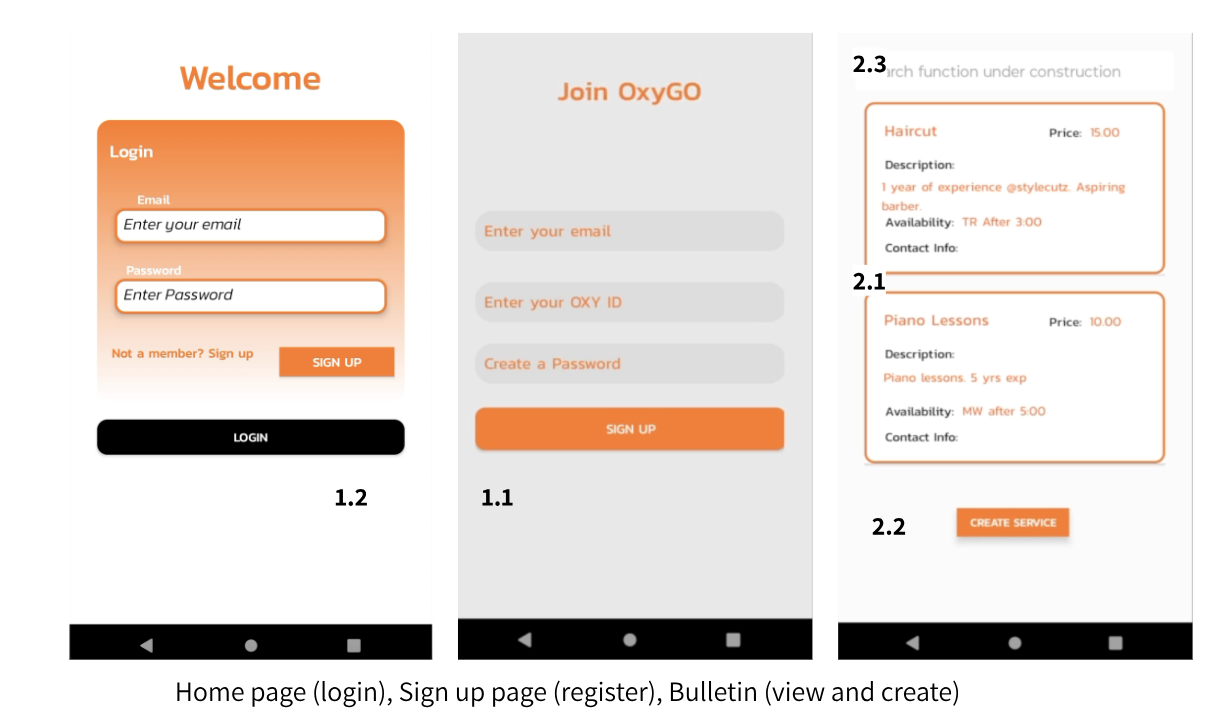
\includegraphics[width=0.5\textwidth]{images/OxyGo.png}
\centering
\end{figure} 

Although specific case studies or user testimonials for OxyGo were not available, similar platforms have demonstrated significant increases in student engagement and campus connectivity. For example, Binghamton University’s partnership with uConnect led to a 153 percent increase in first-year student engagement cite{UConnect}. OxyEvents aims to replicate this success by enhancing campus event discovery and participation.

The development of OxyGo served as a great base for OxyEvents. Since both applications required similar features like user registration and a digital hub for listing events/services, the knowledge gained from OxyGo's design will significantly expedite the development process of OxyEvents. The user profile management, authentication systems, and intuitive interface principles learned from OxyGo can be seamlessly integrated into OxyEvents, ensuring consistency for Occidental College students.

\begin{figure}[h!]
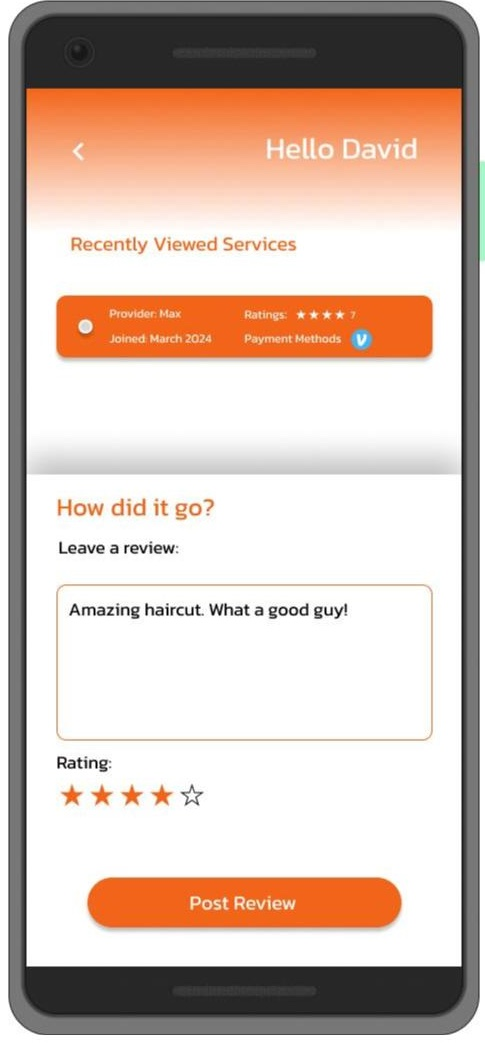
\includegraphics[width=0.5\textwidth]{images/OxyGo(UserProfile).jpg}
\centering
\end{figure} 

Moreover, the backend systems and API integrations established for OxyGo provided a solid foundation for OxyEvents' real-time event data retrieval. Specifically OxyGo's user registration and authentication systems ensure a secure and personalized user experience, which will be adapted for OxyEvents. The backend infrastructure, capable of handling real-time data retrieval and updates, will be crucial for managing dynamic event listings on OxyEvents. By leveraging the existing infrastructure and best practices from OxyGo, there could be more focus on enhancing the unique aspects of OxyEvents specifically to the campus event management and community interaction requirements.

\begin{figure}[h!]
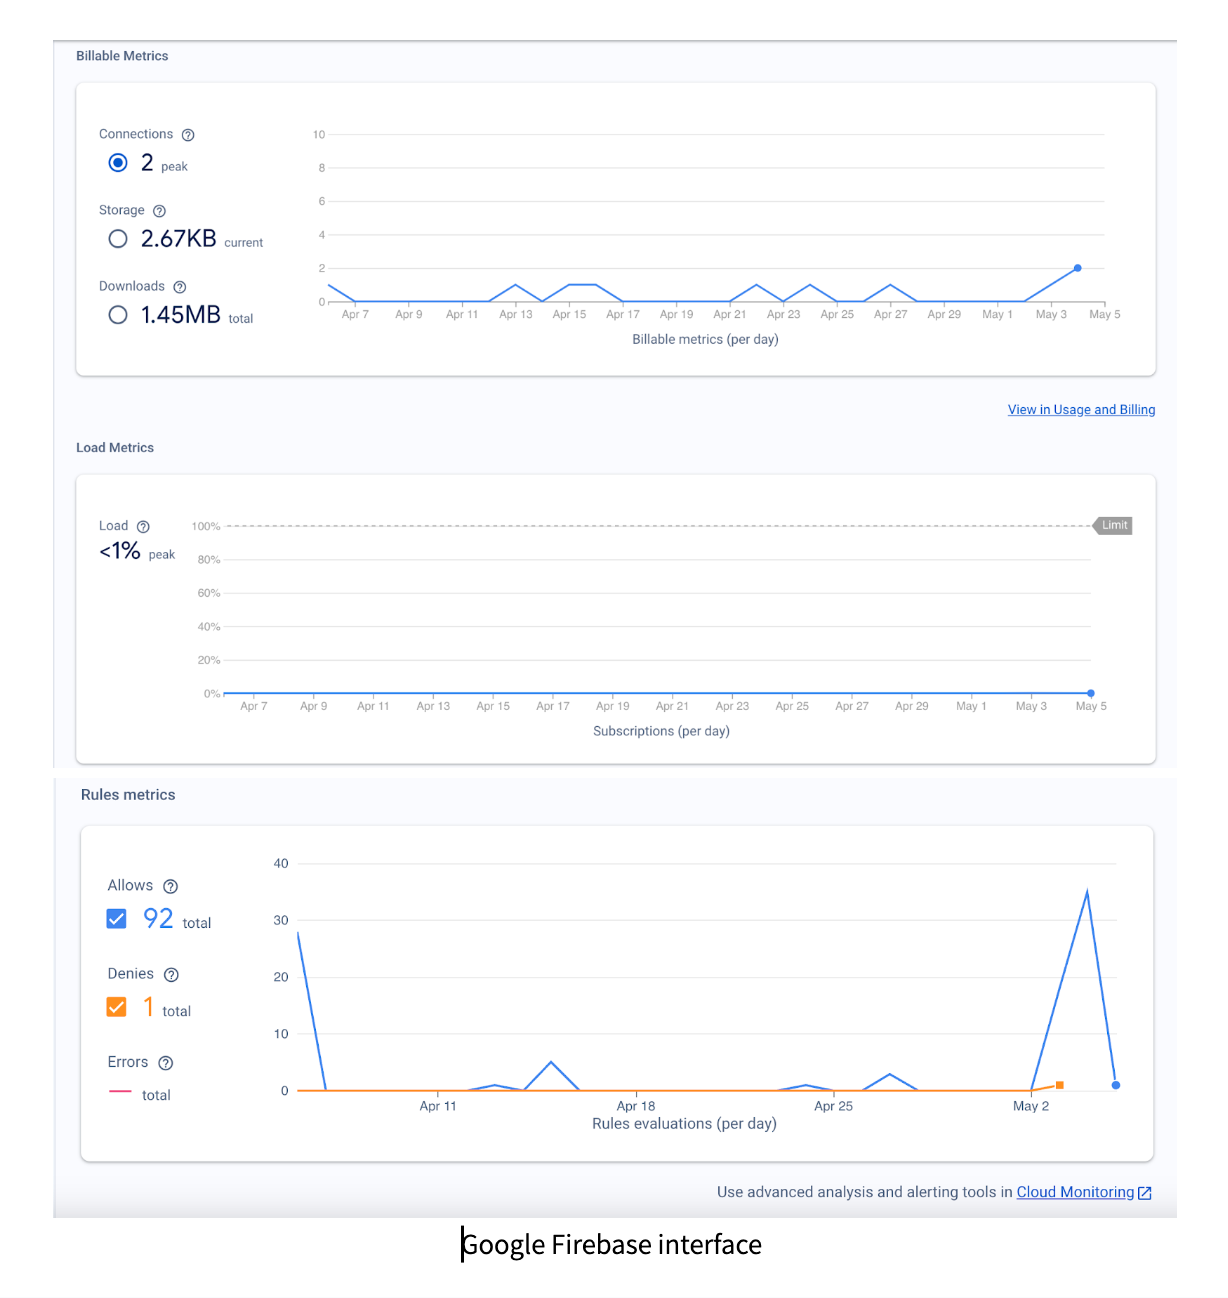
\includegraphics[width=0.5\textwidth]{images/Firebase.png}
\centering
\end{figure} 

The success of OxyGo in empowering students to monetize their skills and connect with peers laid the groundwork for OxyEvents to further enhance campus connectivity and engagement through seamless event discovery, RSVP functionalities, and personalized event tracking. This similarity between OxyGo and OxyEvents showcases a cohesive approach in leveraging technology to enrich the campus experience and foster a vibrant community within Occidental College.

\begin{figure}[h!]
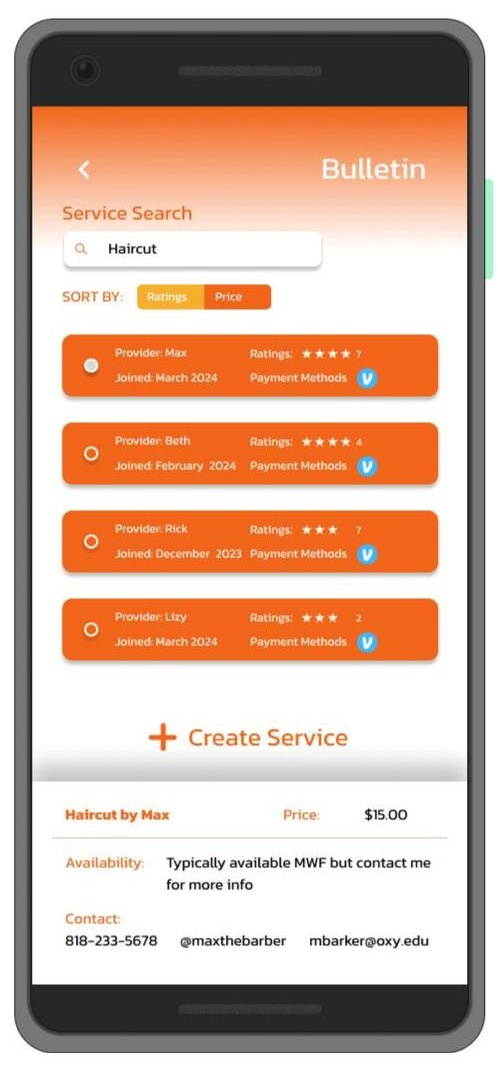
\includegraphics[width=0.5\textwidth]{images/OxyGo(Bulletin).jpg}
\centering
\end{figure} 

\section{Methods} 
The development approach for OxyEvents encompasses several key phases, including backend setup, frontend design, API integration, user profile management, event listing, recommendation algorithms (What’s Hot), and feedback mechanisms. The general flow of information within the app begins with user authentication and profile creation, followed by event data retrieval and presentation based on user preferences and campus relevance. For data preprocessing, we employ techniques such as data cleaning, normalization, and feature extraction to ensure data accuracy and relevance when scraping. 

The methodology for scraping data from Occidental College’s master calendar is a critical component of the OxyEvents app, ensuring that event information is accurate and up-to-date. Will have to employ a combination of automated and manual scraping techniques to extract event data. The process begins with identifying the structure of the master calendar’s web pages and the specific HTML elements that contain event details. 

Can potentially use Python’s calendar module for handling date-based data, which simplifies the process of looping through each day, month, and year to extract relevant information \cite{PythonScrape}. This module accounts for variations in month lengths and leap years, ensuring comprehensive data coverage. Additionally, able to utilize web scraping tools like Octoparse or Import.io, which allow us to extract data without extensive coding\cite{MediumWebScraping101}. For more complex tasks, we may write custom scripts using libraries such as Beautiful Soup in Python\cite{PromptCloud}, which offers fine-grained control over the scraping process.

Once the data is extracted, it undergoes preprocessing steps including data cleaning, normalization, and feature extraction. This ensures that the data fed into the OxyEvents app is reliable and structured, facilitating efficient event listing and recommendation algorithms.
 

The backend setup for OxyEvents is powered by Node.js \cite{Node}, chosen for its efficiency in handling asynchronous events and its non-blocking I/O model, making it ideal for real-time applications that are both data-intensive and scalable. For the frontend, React Native is our framework of choice to ensure a seamless cross-platform experience, leveraging its vast ecosystem and the ability to dip into native performance when needed \cite{ReactNative}. Alternatively, Flutter could be considered for its rapid rendering and expressive UI capabilities, especially if a quicker time-to-market for simpler applications is a priority\cite{FluttervsReact}. Integrating these with a real-time relational database , we utilize GraphQL \cite{GraphQL} as a query language due to its efficient and structured data access, which simplifies the development process and enhances the app’s performance by providing real-time updates and a single endpoint for various types of queries and mutations. This technological combined effort is designed to foster an engaging and intuitive user experience, streamline event management, and enhance community interaction within the Occidental College campus.

\section{Evaluation Metrics}
The evaluation of OxyEvents will be multifaceted, focusing on user feedback, app performance, and engagement metrics \cite{UXMetric}. User surveys and interviews will gather qualitative feedback on usability, satisfaction, and feature preferences. Quantitative metrics such as app retention rates, daily active users, event RSVPs, and user interactions (e.g., comments, shares) will gauge user engagement and app popularity. A/B testing may also be employed to compare different app versions or feature implementations to determine optimal user experiences.

\section{Ethical Considerations}
The OxyEvents app is projected to offer a seamless communication experience by listing all events being held on campus to foster community building and enhances student experiences through reviews of the events. However, when designing event networking apps a delicate balance between innovation and ethical consideration is required.\cite{Appedus}

\section{Data Privacy and Consent}
One of the first areas of concern for campus mobile apps is data and privacy consent. These apps often depend on user data, ranging from personal information to event attendance and preferences. Institutions should be cautious that these applications are providing informed consent, transparency in data usage, and robust security measures.\cite{Appedus}\cite{UofW_IT}\cite{ANA_MobileMarketing}
Informed consent requires that users are fully aware of what data is being collected, how it will be used, and with who it may be shared. One approach for the Campus Events app will be to implement clear and accessible privacy policies, obtain explicit consent from users before collecting sensitive data, and provide mechanisms for users to control their privacy settings.
Transparency is another aspect, as institutions with the OxyEvents app will have to clearly communicate with users on their data collection through the app and its usage practices. This could include informing users about third-party data sharing, data retention policies, and the reasons for which their data will be manipulated.
Security measures, additionally, need to be robust to protect user data from unauthorized access, breaches, and misuse. For the OxyEvents App this will include ensuring that it is with compliance with data protection regulations.

\section{Inclusivity and Accessibility}
While at first glance a OxyEvents mobile app might offer convenience and efficiency, they also raise concerns regarding inclusivity and accessibility. The OxyEvents mobile app is currently being developed for androids in android studios. This could be an issue of inclusivity because not all students will have equal access to android devices. 
To address these concerns, institutions using the OxyEvents app will potentially have to strive for alternative access options for students without androids in order to bridge the digital divide. For example, this could include the institution offering compatible devices on loan for use.
Accessibility should also be considered, as campus apps must be designed to accommodate students with disabilities. This could mean ensuring that the OxyEvents app is withholding to standards like the WCAG (Web Content Accessibility Guidelines)\cite{WCAG}, providing alternative formats for content, and having compatibility with assistive technologies.

\section{Student Health: Balancing Personalization and Privacy}
Mobile applications being implemented in school settings has the potential to impact student well-being and mental health\cite{UofW_IT}. Due to this, the use of OxyEvents app poses ethical challenges related to privacy, notifications, and potential social pressure.
Privacy concerns come from the collection of sensitive data like location and behavioral analytic information, which are often used to personalize app experiences. The OxyEvents app will have to strike a balance between offering personalized features and respecting students privacy rights. This could be done through various design methods including minimizing data collection to what is strictly necessary and allowing for opt-out features for certain data processing activities.\cite{ANA_MobileMarketing}
Notifications are another area of ethical concern because of the risk of excessive/ intrusive notifications contributing to app-induced stress or anxiety.\cite{Appedus} The OxyEvents app should provide users with control over notification settings in order to accommodate to their needs and preferences.
Social pressure within mobile apps that use social features can also impact student health by creating feelings of inadequacy, FOMO (fear of missing out), or social comparison. The OxyEvents app will feature a comment/review activity that will need to comply with certain regulations so that the activity will promote positive interactions, create a supportive community, and discourage negative behaviors contributing to social pressures or cyberbullying.

\section{Distraction}
Additionally while a OxyEvents app may offer a wide range of functionalities, it also has the potential to distract students from academic responsibilities. Therefore, ethical considerations in this context circle around balancing app features, usage limits, and promotion of responsible app usage during study hours.
The OxyEvent app should prioritize academics over social features, ensuring that the app is able to support student success. This could mean integrating a filter that displays events based on academic relevance, like having lecture seminars and guest-speaker events shown before sports/ student club events. Another filter could integrate a student's course schedule and remove events that overlap from the display. 
Setting usage limits can also help mitigate distraction by providing a way for students to manage their app usage effectively. The OxyEvents app will need to include features like app usage analytics to tell students if they've been on the app too much recently or provide additional time management tools.
With the OxyEvents app utilizing a learning-centered design approach, institutions can expect events to promote student success and minimize distractions from academics.\cite{Appedus}

\section{Responsible Data Usage}
In addition to privacy concerns, institutions should also be wary of ethical principles related to data usage. These principles include anonymization of data, research ethics, and making sure data is used in accordance with privacy norms.
The OxyEvents app is meant to improve student life on campus, and in order to protect user privacy while still allowing for data analysis and insights, anonymization of data could be essential. Anonymization of data could be implemented through techniques such as data aggregation, pseudonymization of some user information like names, and forms of de-identification to ensure that student identities are not compromised. 
Research Ethics could play a role in how the app data is used for event research purposes. Institutions will have to adhere to some ethical guidelines established by OxyEvents in order to obtain appropriate user data. This could include obtaining informed consent from users about data collection, ensuring data anonymization and complying with other requirements like institutional review board (IRB).
Without upholding responsible data usage practices, OxyEvents app could have a difficult time providing services, conducting research, and enhancing student life because students don't feel their privacy rights are respected. 

\section{Social Responsibility: Campus Culture}
Mobile apps can play a role in shaping campus culture and social interactions. This raises ethical considerations related to promoting positive interactions, preventing harm, and creating a respectful and inclusive community.
Institutions should prioritize features and functionalities within apps that promote respectful communication, collaboration, and community engagement. For the OxyEvents app facilitating support networks/events and promoting diversity and inclusion initiatives are examples.
Preventing harm within app environments involves implementing policies and mechanisms to address issues such as cyberbullying, harassment, or inappropriate behavior. Institutions must have clear guidelines, reporting mechanisms, and disciplinary measures in place to respond effectively to harmful conduct within app communities.
By promoting social responsibility within app ecosystems, institutions can create a positive and supportive campus culture that enhances student well-being, fosters meaningful connections, and contributes to a healthy learning environment.

\section{Too Risky?}
In essence, while a campus events app may offer convenience and centralization of event information, its unintended consequences in terms of information overload, social pressure, marginalization, and data privacy risks underscore why careful consideration and ethical safeguards are essential before implementing such a tool like OxyEvents within a university or college environment.


\section{Timeline}
\begin{itemize}
    \item Weeks 1-2: Set up development environment, finalize database schema, implement user authentication.
    
    \item Weeks 3-4: Design frontend UI/UX prototypes, integrate basic event listing functionality.
    
    \item Weeks 5-6: Develop user profile management features, implement event filtering and sorting options. 
    
    \item Weeks 7-8: Integrate API for real-time event data retrieval, start implementing recommendation algorithms.
    
    \item Weeks 9-10: Fine-tune recommendation algorithms, add RSVP and reminder functionalities.
    
    \item Weeks 11-12: Implement feedback mechanisms, conduct user testing and feedback collection.
    
    \item Weeks 13-14: Finalize app features, conduct performance testing, prepare for final comps paper submission.
    
\end{itemize}

\printbibliography

\end{document}
